\documentclass[12pt]{standalone}

% Commands for writing shorthand lattice operators
\newcommand{\MU}{\hat{\mu}}
\newcommand{\NU}{\hat{\nu}}


\usepackage{tikz}

\usetikzlibrary{decorations.markings}
\usetikzlibrary{math}

\begin{document}
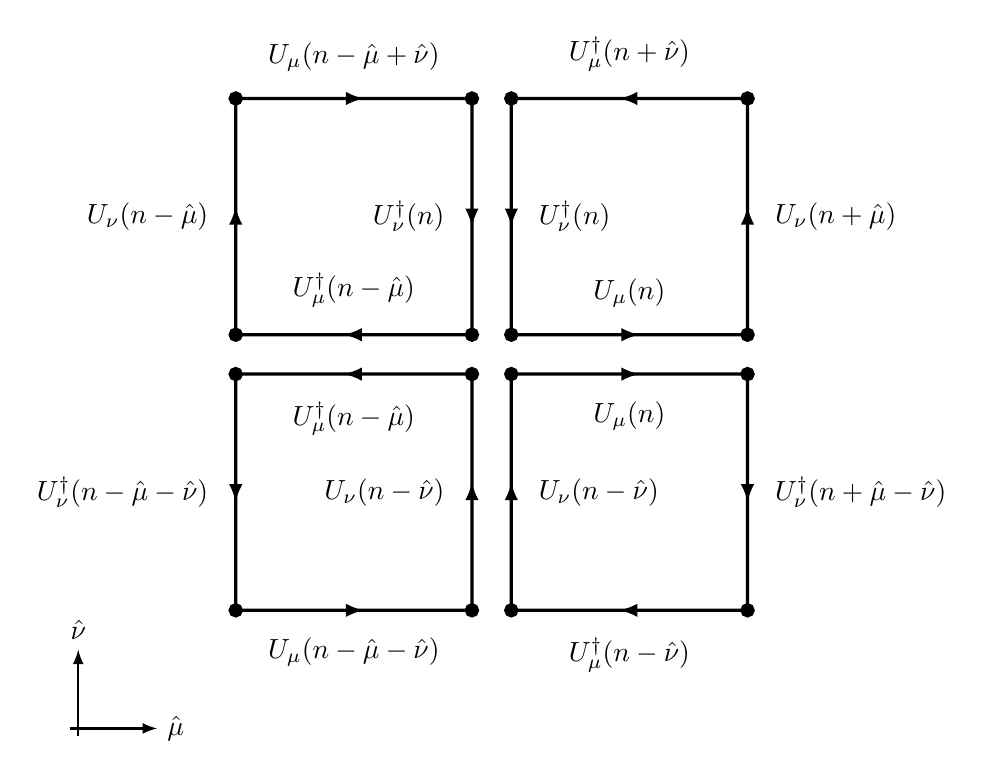
\begin{tikzpicture}

% Position settings
\tikzmath{
    \LinkLength = 3;
    \StapleXShift = 0.5 + \LinkLength;
    \StapleYShift = 0.5;
    \AxesShift = 3.5;
}

\coordinate (C1X0) at (0,0);
\coordinate (C1X1) at (\LinkLength, 0);
\coordinate (C1X2) at (\LinkLength, \LinkLength);
\coordinate (C1X3) at (0, \LinkLength);

\coordinate (C2X0) at (0, -\StapleYShift);
\coordinate (C2X1) at (\LinkLength, -\StapleYShift);
\coordinate (C2X2) at (\LinkLength, -\LinkLength - \StapleYShift);
\coordinate (C2X3) at (0, -\LinkLength - \StapleYShift);

\coordinate (C3X0) at (-\StapleXShift, 0);
\coordinate (C3X1) at (\LinkLength - \StapleXShift, 0);
\coordinate (C3X2) at (\LinkLength - \StapleXShift, \LinkLength );
\coordinate (C3X3) at (-\StapleXShift, \LinkLength);

\coordinate (C4X0) at (-\StapleXShift, -\StapleYShift);
\coordinate (C4X1) at (\LinkLength - \StapleXShift, -\StapleYShift);
\coordinate (C4X2) at (\LinkLength - \StapleXShift, -\LinkLength - \StapleYShift);
\coordinate (C4X3) at (-\StapleXShift, -\LinkLength - \StapleYShift);


\begin{scope}[very thick,decoration={
    markings,
    mark=at position 0.6 with {\arrow{latex}}},
    ] 

    % First clover
    \draw [black, very thick, fill, postaction={decorate}]
        (C1X0) circle (2pt) -- node [midway,above=6pt] {$U_\mu(n)$} (C1X1);
    \draw [black, very thick, fill, postaction={decorate}]
        (C1X1) circle (2pt) -- node [midway,right=6pt] {$U_\nu(n+\MU)$} (C1X2);
    \draw [black, very thick, fill, postaction={decorate}]
        (C1X2) circle (2pt) -- node [midway,above=6pt] {$U_\mu^\dagger(n+\NU)$} (C1X3);
    \draw [black, very thick, fill, postaction={decorate}]
        (C1X3) circle (2pt) -- node [midway,right=6pt] {$U_\nu^\dagger(n)$} (C1X0);

    % Draws second clover
    \draw [black, very thick, fill, postaction={decorate}]
        (C2X0) circle (2pt) -- node [midway,below=6pt] {$U_\mu(n)$} (C2X1);
    \draw [black, very thick, fill, postaction={decorate}]
        (C2X1) circle (2pt) -- node [midway,right=6pt] {$U_\nu^\dagger(n+\MU-\NU)$} (C2X2);
    \draw [black, very thick, fill, postaction={decorate}]
        (C2X2) circle (2pt) -- node [midway,below=6pt] {$U_\mu^\dagger(n-\NU)$} (C2X3);
    \draw [black, very thick, fill, postaction={decorate}]
        (C2X3) circle (2pt) -- node [midway,right=6pt] {$U_\nu(n-\NU)$} (C2X0);

    % Third clover
    \draw [black, very thick, fill, postaction={decorate}]
        (C3X1) circle (2pt) -- node [midway,above=6pt] {$U^\dagger_\mu(n-\MU)$} (C3X0);
    \draw [black, very thick, fill, postaction={decorate}]
        (C3X0) circle (2pt) -- node [midway,left=6pt] {$U_\nu(n-\MU)$} (C3X3);
    \draw [black, very thick, fill, postaction={decorate}]
        (C3X3) circle (2pt) -- node [midway,above=6pt] {$U_\mu(n-\MU+\NU)$} (C3X2);
    \draw [black, very thick, fill, postaction={decorate}]
        (C3X2) circle (2pt) -- node [midway,left=6pt] {$U^\dagger_\nu(n)$} (C3X1);

    % Fourth clover
    \draw [black, very thick, fill, postaction={decorate}]
        (C4X1) circle (2pt) -- node [midway,below=6pt] {$U^\dagger_\mu(n-\MU)$} (C4X0);
    \draw [black, very thick, fill, postaction={decorate}]
        (C4X0) circle (2pt) -- node [midway,left=6pt] {$U^\dagger_\nu(n-\MU-\NU)$} (C4X3);
    \draw [black, very thick, fill, postaction={decorate}]
        (C4X3) circle (2pt) -- node [midway,below=6pt] {$U_\mu(n-\MU-\NU)$} (C4X2);
    \draw [black, very thick, fill, postaction={decorate}]
        (C4X2) circle (2pt) -- node [midway,left=6pt] {$U_\nu(n-\NU)$} (C4X1);
\end{scope}

% Draws axis
\draw [black, thick, -latex] (-2.1-\AxesShift,-1.5-\AxesShift) -- (-1-\AxesShift,-1.5-\AxesShift) node [right] {$\hat{\mu}$};
\draw [black, thick, -latex] (-2-\AxesShift,-1.6-\AxesShift) -- (-2-\AxesShift,-0.5-\AxesShift) node [above] {$\hat{\nu}$};



\end{tikzpicture}
\end{document}
